% Three Streams: mixing a conversational model's context with certified inference — draft 0.1
% Build: tectonic streams.tex   (references in streams.bib; the sibling papers' preamble)
\documentclass[11pt]{article}

\usepackage[a4paper,margin=1.1in]{geometry}
\usepackage{amsmath,amssymb}
\usepackage{lmodern}
\usepackage{microtype}
\usepackage{booktabs}
\usepackage{array}
\usepackage{enumitem}
\usepackage{xcolor}
\usepackage{tikz}
\usetikzlibrary{positioning,arrows.meta,fit,calc}
\definecolor{linkblue}{rgb}{0.1,0.15,0.45}
\usepackage[colorlinks=true,linkcolor=linkblue,citecolor=linkblue,urlcolor=linkblue]{hyperref}
\usepackage{cmap}
\emergencystretch=3em

% ---- notation (the sibling papers') -----------------------------------------
\newcommand{\llp}{\textsc{llp}}
\newcommand{\metisc}{\texttt{metisc}}
\newcommand{\metispy}{\texttt{metispy}}
\newcommand{\agent}{\texttt{metis-agent}}
\newcommand{\fsttm}{\textsc{fsttm}}
\newcommand{\orgurl}{\url{https://github.com/metis-lang-dev}}
% a source pointer: the document, file or commit a statement comes from
\newcommand{\src}[1]{{\footnotesize\textsf{[#1]}}}
% the status of a claim: built (code exists and is tested), observed (a small
% measurement or a transcript), proposed (designed, not built)
\newcommand{\built}{\textsf{\small[built]}}
\newcommand{\observed}{\textsf{\small[observed]}}
\newcommand{\proposed}{\textsf{\small[proposed]}}
\newcommand{\todo}[1]{{\color{red}\textsf{\small[TODO: #1]}}}

\title{\textbf{Three Streams}\\[1ex]
\large Mixing a conversational model's context with the inference of a certified rule
engine, in a home}
\author{The metis project\thanks{Sources: the \fsttm{} branch \texttt{cloud-llm}
(\url{https://github.com/ibnHatab/FSTTM}), the acasa repository (design
\texttt{docs/DIALOG-METIS.md}), and \agent{} with its sibling repositories at \orgurl.
Correspondence: \texttt{info@robofortis.com}.}}
\date{Draft 0.1 --- 2026-11-21}

\begin{document}
\maketitle

\begingroup\small\noindent
\textbf{How to read this draft.} It reports one day of building, so most of it is design.
Every statement is marked: \built{} --- the code exists and its tests pass;
\observed{} --- a small measurement or a recorded transcript, with $n$ stated, never a
benchmark; \proposed{} --- designed in \texttt{DIALOG-METIS.md}, not built. Numbers carry a
pointer \src{source} to the commit or document they come from. The sibling papers are
\emph{Behavior Programs as Measures over Proofs} (the language, draft 0.5),
\emph{Behavior Catalogs in Practice} (the catalog and the loop, draft 0.3) and
\emph{Small Models, Certified Behavior} (the on-device agent, draft 0.3); this one changes
the setting they share in one respect --- the model is no longer small, local and
grammar-bound, but a cheap cloud model in free conversation.
\endgroup

\begin{abstract}
A conversational language model in a home is asked about things it cannot see and to do
things it cannot check: whether the light is on, whether the heating was turned on, why the
fan is running. A small or cheap model answers anyway. The sibling paper on the on-device
agent gave the model less authority: a certified behavior runtime owns state, procedure and
legality, and the model maps words to typed intents. This paper keeps that division but lets
the model talk freely. The model --- Gemini 3.1 Flash-Lite behind an OpenAI-compatible API,
driven by the \fsttm{} turn-taking engine --- is told in its system prompt that it works with
\emph{three parallel streams}: the CONVERSATION, the only stream addressed to it; the
ENVIRONMENT, the home's state as Home Assistant reports it; and the REASONING, the
conclusions of the metis rule engine, a separate process running beside the conversation.
The two non-conversational streams enter the context as timestamped, overwritten or
appended entries, never as turns. The model is told an authority order --- environment over
reasoning over its own belief --- and that a request to change the home is decided by the
rule engine while it speaks, so it may say it is on it but never that it is done until the
outcome is in REASONING. We describe the design and what is built (the streams, a local door
for producers, a Home Assistant feed, a panel), report preliminary observations from a
handful of scripted probes on the live system (one completion claim before the prompt said
when an outcome may be claimed, none after; correct answers from real Home Assistant state
with one omission), and propose the evaluation that would test the claim we actually care
about: that injecting a rule engine's inferences into a cheap model's context makes its
answers and its actions more correct than the model alone.
\end{abstract}

\section{Introduction}\label{sec:intro}

A voice assistant in a home has two kinds of knowledge it does not hold. The first is the
\emph{state of the world}: the devices, the sensors, who is in which room. The second is
\emph{what follows from it under the household's rules}: that a request was refused and why,
that nobody is home and the lights are still on, that the ventilation should not boost at
night. A language model holds neither. A small or cheap one, asked anyway, produces a
fluent guess, and the guess is worst exactly where it matters: it reports actions as done
that were never taken, and states as observed that were never read
(\cite{ji2023survey} survey the phenomenon in general; the sibling agent paper measures it
for one small model: E10, the response turn ``invites completion claims'').

The sibling paper's answer was to give the model less authority \src{agent paper
\S1}: a behavior program in \llp{} owns state, procedure, probability and safety; the model
gets narrow, checked jobs --- map an utterance to one typed intent, narrate, propose an
explanation, ask. That answer assumes the model is the device's front: every utterance is
an intent or a refusal. In a home it is not. Most of what is said is conversation, some of
it is about the home, and a little of it asks the home to act. A free-running conversational
model is the right front for that; a grammar-bound intent mapper is not.

This paper asks how to keep the certified side in charge of state and action while the model
talks freely. Our answer is a context discipline we call \emph{three streams}:

\begin{enumerate}[nosep]
\item \textbf{CONVERSATION} --- the person's words (from speech recognition) and the model's
replies. The only stream addressed to the model; the only one it answers.
\item \textbf{ENVIRONMENT} --- the home's state as the device platform reports it (Home
Assistant), keyed by entity, a newer reading replacing the older. The truth about devices.
\item \textbf{REASONING} --- the conclusions of the rule engine (metis), appended in time
order: an outcome (done, refused and why), an inference, a thing it noticed. A separate
reasoning process that runs in parallel with the model and the conversation.
\end{enumerate}

\noindent The model is told what each stream is, how far to trust it, and what it may claim
before the rule engine has decided. The contribution is not the idea of putting state in a
prompt --- retrieval-augmented generation \cite{lewis2020rag} and every tool-using agent
\cite{yao2023react,schick2023toolformer} do that --- but three specific choices:
(i)~\emph{inference, not retrieval}: what enters is a certified engine's conclusions, with
their reasons, not documents; (ii)~\emph{streams, not turns}: the entries never become
messages in the dialog, so the model never answers them and never mistakes them for the
person; (iii)~\emph{an explicit authority order and an explicit claim rule} in the prompt,
so a cheap model can be told, in words, where its own beliefs stop.

\section{The setting}\label{sec:setting}

The system runs on an Intel NUC (i3-10110U, two cores, 7\,GB, no GPU) in a flat \observed{}.

\begin{description}[nosep,leftmargin=1.2em]
\item[Voice.] \fsttm{}, an implementation of the finite-state turn-taking model of Raux and
Eskenazi \cite{raux2009fsttm}, with barge-in: a ReSpeaker 4-mic array (its processed,
echo-cancelled channel), voice activity detection, Whisper \cite{radford2023whisper}
(\texttt{base.en}, CPU) for speech recognition, Piper for speech \built.
\item[Model.] Gemini 3.1 Flash-Lite through Google's OpenAI-compatible endpoint, by a new
\fsttm{} backend (\texttt{fsttm/cloud.py}) that speaks the engine's existing message protocol
over \texttt{chat/completions}: streamed chat with a FIFO history, cancellation by closing the
stream \built{} \src{FSTTM e0a9466}. The same backend reaches OpenRouter or a
\texttt{llama-server} by base URL.
\item[Devices.] Home Assistant in a container: two Prana recuperators (supply and extract
fans with speed and presets, heater and mode switches, an outside-temperature sensor each),
a television, a light; planned: an mmWave presence radar, Bluetooth thermometers, a USB
infrared transmitter \observed.
\item[Rules.] A metis catalog domain for the home: \llp{} rules with \texttt{\%\%} narration
lines, an \texttt{intent.yaml} grounding contract, a host that reads and drives the devices
\built{} for a first four-device domain \src{acasa \texttt{domains/home}; c603549}; the full
home world is being written as this draft is.
\end{description}

\paragraph{Why not the on-device agent unchanged.} The sibling paper's agent ran on this NUC
first, with Gemma~4~E2B on the CPU. A switch command took about 13\,s from words to spoken
reply; removing the consult seat and the domain narrator and shortening the intent JSON from
about 35 to 12 generated tokens brought it to about 7\,s \observed{} \src{acasa 4b700e3,
c603549; three to six scripted turns per configuration}. The Go backend with the same llama.cpp
measured the same on this CPU \observed{} \src{acasa c603549, README}: the limit is the
token rate (about 10 tokens/s), not the language. Gemini 3.1 Flash-Lite from the same NUC
answered a one-sentence prompt in 2.5--3.5\,s by default and 1.6--1.8\,s with thinking turned
off \observed{} \src{FSTTM d89dfc0; $n=2$ each}. With a thinking level of ``low'' and a
100-token cap, the thinking consumed the budget and the visible reply was cut to one word
\observed; a local \texttt{llama-server} with Gemma~4 and thinking on returned an empty first
reply for the same reason, which is why the backend now reports a thinking-only reply as an
error with the remedy \built{} \src{FSTTM e0a9466}. On the voice side, Whisper \texttt{base.en}
transcribed 3.8\,s of speech in 2.2\,s and \texttt{tiny.en} in 1.0\,s; Piper rendered it in
0.26\,s \observed{} \src{FSTTM 48122bf; one utterance}. The cloud model is therefore the
latency choice on this hardware; it is also the reason the design below must not trust it.

\section{Three streams}\label{sec:streams}

\begin{figure}[t]
\centering
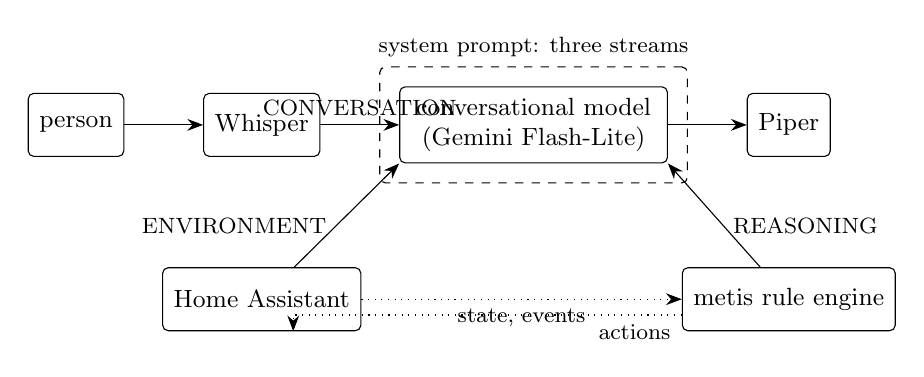
\begin{tikzpicture}[node distance=6mm and 10mm, every node/.style={font=\small},
  box/.style={draw, rounded corners=2pt, align=center, inner sep=4pt, minimum height=8mm},
  arr/.style={-{Stealth[length=2mm]}}]
\node[box] (person) {person};
\node[box, right=of person] (stt) {Whisper};
\node[box, right=of stt, minimum width=34mm] (llm) {conversational model\\(Gemini Flash-Lite)};
\node[box, right=of llm] (tts) {Piper};
\node[box, below=14mm of stt] (ha) {Home Assistant};
\node[box, below=14mm of tts] (metis) {metis rule engine};
\node[draw, dashed, rounded corners=2pt, fit=(llm), inner sep=7pt, label={[font=\footnotesize]above:system prompt: three streams}] {};
\draw[arr] (person) -- (stt);
\draw[arr] (stt) -- node[above, font=\footnotesize]{CONVERSATION} (llm);
\draw[arr] (llm) -- (tts);
\draw[arr] (ha) -- node[left, font=\footnotesize, pos=0.4]{ENVIRONMENT} (llm.south west);
\draw[arr] (metis) -- node[right, font=\footnotesize, pos=0.4]{REASONING} (llm.south east);
\draw[arr, dotted] (ha) -- node[below, font=\footnotesize]{state, events} (metis);
\draw[arr, dotted] (metis.west) ++(0,-2mm) -- ++(-12mm,0) node[below, font=\footnotesize, pos=0.5]{actions} -| ([xshift=4mm]ha.south);
\end{tikzpicture}
\caption{The three streams. Only CONVERSATION is a dialog; ENVIRONMENT and REASONING enter
the model's system prompt as timestamped entries. Dotted: the rule engine reads the devices'
state and acts through Home Assistant (the action path is \proposed).}
\label{fig:streams}
\end{figure}

\subsection{What is built}

The backend keeps two stores beside the dialog history \built{} \src{FSTTM d26d480,
\texttt{fsttm/cloud.py}}: the ENVIRONMENT as a map from entity to its latest line and time
(a new entry replaces the old; a null text removes the entity), and the REASONING as a
bounded queue of the last twelve conclusions with their times. On every request the system
prompt is rebuilt from three parts: the persona, a fixed explanation of the streams
(\texttt{STREAMS\_PROMPT}, quoted in Appendix~\ref{app:prompt}), and the two stores rendered
as lists --- \texttt{ENVIRONMENT (as of 20:31:02):} one line per entity, \texttt{REASONING
(newest last):} one line per conclusion. The message list sent to the API stays
\emph{system, user, assistant, \dots, user}; a test checks that the streams never add a
message \built{} \src{\texttt{tests/test\_cloud\_llm.py}}.

Producers are separate processes. A local TCP port (the \emph{stream door}) takes one JSON
object per line --- \texttt{\{"stream": "env", "key": "fan.lab\_supply\_fan", "text": "lab
Supply fan: off"\}} --- and the engine routes each to the backend as a non-turn event
\built{} \src{\texttt{fsttm/streams.py}}. The Home Assistant feed reads every state once over
Home Assistant's websocket API, then follows \texttt{state\_changed}, writing an entity's line
only when its words change \built{} \src{FSTTM d2497a6}. A panel on a second port shows the
three streams in separate columns for a screen beside the dashboard \built{} \src{FSTTM
ea4a165}. The REASONING producer --- the metis sidecar --- was built after the observations reported here (FSTTM \texttt{8293ba8}, \texttt{fsttm-metis}: the domain agent over the home world's packages, its outcomes into REASONING and its packages as the model's tools; \S\ref{sec:future});
in the observations below its entries were scripted.

\subsection{Why streams and not turns}

The obvious way to give a chat model new facts is to send them as messages: a tool result, a
``system'' turn, a user turn that says ``FYI''. Three things go wrong with that, and the
sibling paper measured two of them on a small model. First, a model answers turns: a fact
sent as a turn is a fact the model replies to, aloud. Second, a response turn carries a
trained prior --- \emph{call, result, done}: in E10, every arm that saw a result turn
reported a task complete on some mere acceptances, and the JSON-text path never did
\src{agent paper \S5.4: E10, 4 completion claims}. Third, a fact in the dialog
ages badly: in E6, a fact spliced into the context did not carry across turns reliably
(0.42--0.75 at six turns), and the newer of two values did not reliably win (0.75 newer
against 0.08 older) \src{agent paper \S5.2: E6/E6b}. E6's ruling --- standing facts go in an
overwritten mirror, not in the history --- is what the ENVIRONMENT store is: one line per
entity, replaced in place, always at the head of the context. The REASONING store is the
part of E6 that changes: conclusions are events, not standing facts, so they are appended,
bounded, and timed, and the prompt says a newer entry supersedes an older.

A cloud model's context is not a KV cache, so the sibling design's other reason for the
mirror --- an append-only tape where past tokens cannot be edited --- does not apply. Here
the system prompt is rebuilt on every request; the cost is input tokens, and the free tier's
rate limits, not latency \observed{} (\S\ref{sec:obs}).

\subsection{Authority, provenance and the claim rule}

The prompt states an order of authority: the ENVIRONMENT is ``the truth about the devices,
more reliable than what you assumed or what the person remembers''; the REASONING ``about
what the home did and can do, is authoritative: when it contradicts what you expected or
said, follow it and correct yourself''; the model's own belief comes last. This mirrors the
evidence rules of the design \src{DIALOG-METIS \S3}: a device reading is the world; a
person's report (``the light is broken'') is an intent that lands as its own atom, compared
by rules with the reading; the assistant's words are never evidence. The last rule is the
one a probabilistic system most needs and a language model most easily breaks: if the
model's restatement of a user's claim were read back as a second observation, the system
would confirm itself. Here it cannot, by construction: no producer reads the conversation's
assistant side into a stream \proposed{} for the observer, \built{} for the two producers
that exist.

The \emph{claim rule} is the part a prompt can do and a protocol cannot: ``You do not switch
anything yourself: a request to change something in the home goes to the rule engine, which
decides it while you speak. Until its outcome is in REASONING, say only that you are on it
--- never that it is done, and never invent a refusal.'' The rule exists because the first
probe broke it (\S\ref{sec:obs}).

\subsection{Asynchronous inference, synchronous authorization}

The model and the rule engine run in parallel: the model never waits for an inference to
speak, and the engine never waits for the model to decide. Two paths cross between them
\src{DIALOG-METIS \S1.1}. The \emph{observation} path is asynchronous: every person turn also
goes to an observer, which extracts what concerns a served domain and feeds it to the
engine; its conclusions arrive in REASONING whenever they arrive \proposed. The
\emph{authorization} path is synchronous where it must be: anything that changes the home
is a typed intent to the engine, whose rules accept or refuse it; the action happens only on
an acceptance \proposed. The claim rule is what lets the conversation stay asynchronous over
a synchronous authorization: the model acknowledges at once, the outcome follows in its own
stream, and the model reports it when asked, or on its own when it was a refusal.

\section{Projecting inference into the context}\label{sec:projection}

What the engine puts into REASONING is chosen so that a cheap model can use it without
interpretation. Three properties of metis make that possible \src{agent paper \S3}:

\begin{description}[nosep,leftmargin=1.2em]
\item[Narration lines are the rules' own words.] Every \llp{} rule carries a \texttt{\%\%}
line --- \texttt{\%\% I can't turn \{D\} on: it does not answer on the network.} --- and the
line of the rule that fired, with its variables bound, is the conclusion's text. The
renderer is deterministic code; no model paraphrases a fact before the conversational model
sees it (the sibling paper's E6 ruling).
\item[Refusals name their blocker.] A refusal is a rule that fired, so its reason is the
blocking atom it rested on, and a host can map that atom to what the person could do
(``check that the TV has power and is on the Wi-Fi'') \built{} \src{acasa
\texttt{domains/home/home\_host.py} \texttt{WORDS}}. The model is handed the remedy, not
asked to invent one.
\item[Beliefs are not observations.] A program declares which predicates the host infers
rather than observes (the manifest's \texttt{belief} list), and its probabilities come from
ports fitted from recorded sessions, never from a model's stated confidence
\src{CATALOG.md; DIALOG-METIS \S0}. A conclusion that rests on a belief can say so.
\end{description}

\noindent This is the difference from retrieval \cite{lewis2020rag}: the context does not
receive passages that might be relevant; it receives the consequences the household's rules
draw from the current state, each with its reason. It is also the difference from tool use
\cite{yao2023react,schick2023toolformer}: the model does not decide when to consult the
engine, and does not interpret a tool's raw output; the engine pushes conclusions, already in
words, into a place the model is told how to treat.

\section{The extraction side: a grounding contract, not a semantic frame}\label{sec:extraction}

For the engine to reason about the conversation, something must turn words into atoms. The
literature offers a rich apparatus: dialog state tracking keeps an evolving representation of
goals and slots across turns \cite{williams2016dstc,henderson2014dstc2}; context-dependent
semantic parsing maps utterances in a conversation to executable forms
\cite{suhr2018context,iyyer2017sqa}; ontology-guided parsing constrains the output to a
schema \todo{a representative ontology-guided semantic parsing reference}. A proposal we were
handed while designing this system suggested an intermediate ``semantic frame''
(dialog act, proposition, polarity, modality, confidence, provenance) that a compiler would
translate into clauses.

In metis that layer already exists, and it is narrower on purpose. A domain's
\texttt{intent.yaml} declares the verbs a person may use, their slots, examples, and the
\emph{handles} that ground a phrase to a catalog name (``bedroom ventilation'', ``bedroom
fan'' $\to$ \texttt{vent\_bedroom}); a deterministic mapper turns a typed intent into one
command atom, with a fallback handle for a name the domain does not know; from the same file
the generator writes the grammar, the prompt and a corpus \src{agent paper \S3;
acasa \texttt{domains/home/intent.yaml}}. The grounding is therefore a contract the
catalog owns, not an output the model invents: the model may only fill the slots, and only
the mapper decides what they mean. Rules are never generated from a turn; a sentence that
proposes a rule (``from now on, never boost at night'') becomes a proposal for the
improvement loop, not an active rule \src{DIALOG-METIS \S8}. Probabilities are never a
model's confidence. Dialog acts map onto existing notions --- a request onto a command
intent, a question onto a query, a report onto a report intent whose rules compare it with
the reading --- and the new piece is the report verb and its agree/dispute rules
\proposed.

\section{The improvement loop}\label{sec:loop}

A rule engine in a home will be wrong in ways nobody wrote down. metis records what its
program did not predict: a reading no run of the program reaches is a \emph{surprise}, with
the program key, the steps, the observed counts, the likelihood and the host's snapshot, so
it replays \src{agent paper \S3}. The conversation adds producers of
surprises --- a name nobody grounded (``the ambient lights''), a report that disputes a
reading, a request no rule covers --- but no new kinds \src{DIALOG-METIS \S5}. Surprises are
written to the domain's workspace; Claude Code, attached to the workspace through the metis
plugin's tools, takes them, proposes a rule or vocabulary change, runs the gate, and commits
on a branch; a person merges \proposed{} (the plugin and the gate are \built{} in the
catalog's repositories \src{catalog paper; metis-agent \texttt{plugin/README.md}}). The
household's assistant thereby improves by changes to its rules that a person approved, never
by retraining, and the conversational model never writes a rule.

\section{Preliminary observations}\label{sec:obs}

All of the following are single runs of a scripted probe (\texttt{scripts/streams\_probe.py})
or one-off questions against the live system; they illustrate behavior and are not evidence
of rates.

\paragraph{The claim rule is needed, and a sentence suffices (n=1 each way).} With the first
version of the prompt, which said only that an outcome ``may be decided by the rule engine
after you reply'', the request ``Turn off the TV, please.'' was answered ``I have turned off
the television for you.'' with nothing in REASONING \observed{} \src{FSTTM 2d14e9d}. With the
claim rule added, the same request was answered ``I am turning off the TV now.''; after a
scripted \texttt{done} entry and the environment's update, ``Did that work?'' was answered
``Yes, the TV is now off.''; ``Turn on the heating, I'm cold.'' was answered ``I am turning on
the heating for you now.'', and after a scripted refusal (``it is not a device I know in this
home''), the next turn corrected it: ``I cannot turn on the heating because it is not a device
I recognize.'' \observed. This is the sibling paper's E10 finding again, in a different model
and format: a model that has been asked to act reports it as done unless told when it may.

\paragraph{Answers from the environment (n=3 questions).} With the 16 entities Home Assistant
reported (two recuperators), ``Is the ventilation running anywhere?'' was answered ``No, the
ventilation is currently off in both the bedroom and the lab.''; ``How warm is it outside?''
with the two sensors' values; ``Which ventilation modes do I have?'' listed the five mode
switches but omitted the fans' night and boost presets, which were in the entries' attributes
\observed. The sensors labelled ``outside temperature'' read 25--28\,$^\circ$C on a November
evening, likely the air inside the stopped units; the model reported them as outside
temperatures. The environment stream is authoritative only as far as its labels are true ---
a limitation of the design, not of the model (\S\ref{sec:limits}).

\paragraph{Latency.} Replies took 0.5--1.8\,s per turn in these probes \observed; speech
recognition (about 2.4\,s per utterance with \texttt{base.en}) dominated the voice loop
\observed{} \src{FSTTM 48122bf}.

\section{Proposed evaluation}\label{sec:eval}

The claim of this paper is not that the streams work in a probe but that a rule engine's
inference, projected into a cheap model's context, makes the model's answers and actions more
correct than the model alone. The design's experiment tests it \proposed{} \src{DIALOG-METIS
\S7.1}: 100 scripted, labelled user turns over the home domain --- 30 requests (10 phrased
indirectly, ``it's too dark in the lab''), 15 queries, 15 reports (5 disputing a reading), 10
corrections and follow-ups, 10 policies or preferences, 5 hypotheticals, 15 off-topic ---
run through \fsttm{} headless with the sidecar on simulated devices, in three conditions:
the model alone; the model with ENVIRONMENT; the model with ENVIRONMENT and REASONING.
Measures:

\begin{enumerate}[nosep]
\item \emph{routing recall}: relevant turns that reached the mapper;
\item \emph{grounding accuracy}: the mapper's atom against the label;
\item \emph{act accuracy}: request, query, report, policy, distinguished;
\item \emph{reasoning gain}: follow-up questions answered correctly (``did I leave anything
on?'', ``why is the fan off?'') across the three conditions;
\item \emph{false-action and false-claim rates}: device actions not preceded by a
\texttt{done} outcome (must be zero by construction) and spoken claims of completion without
one, with and without REASONING and the claim rule;
\item \emph{latency and cost}: words to reply, p50/p95, and API calls per turn.
\end{enumerate}

\noindent The output is a golden-style record, so a later change to the rules or the prompt
is compared turn by turn. A second experiment varies the model (Gemini Flash-Lite against a
role-play model on OpenRouter and the local Gemma~4 E2B) with the streams held fixed, to
separate what the streams contribute from what the model brings.

\section{Related work}\label{sec:related}

\textbf{Tool-using agents.} ReAct \cite{yao2023react} interleaves a model's reasoning with
actions it chooses; Toolformer \cite{schick2023toolformer} teaches a model when to call. In
both the model owns the loop. Here the engine owns the decision and pushes its conclusions;
the model chooses words, not actions. \textbf{Grounded robotics.} SayCan \cite{ahn2022saycan}
scores a model's proposals by what a robot can do; Inner Monologue \cite{huang2022inner}
feeds environment feedback back into the model's prompt as text --- the closest relative of
the ENVIRONMENT stream; we add a separate, authoritative inference stream and an explicit
claim rule. \textbf{Models and planners.} LLM+P \cite{liu2023llmp} hands planning to a
classical planner; the LLM-Modulo position \cite{kambhampati2024llmmodulo} argues that a model
should propose and external verifiers should check --- the division this paper and its
siblings implement, with a probabilistic linear-logic program \cite{girard1987linear} in the
verifier's place. \textbf{Probabilistic logic.} Markov logic \cite{richardson2006mln} attaches
weights to first-order formulas; metis's programs denote measures over their own runs
(the language paper) and are evaluated exactly. \textbf{Dialog.} Turn-taking is
\cite{raux2009fsttm}; dialog state tracking \cite{williams2016dstc} and context-dependent
semantic parsing \cite{suhr2018context} are the extraction side we replace with a catalog
contract. \textbf{Retrieval.} RAG \cite{lewis2020rag} puts retrieved text in context; we put
inferred consequences. \textbf{Linear logic for interactive worlds.} Ceptre
\cite{martens2015ceptre}.

\section{Limitations}\label{sec:limits}

The REASONING producer is not built; every REASONING entry in \S\ref{sec:obs} was scripted.
The probes are single runs; a cloud model's answers vary between runs, and nothing here
estimates a rate. A prompt is a request, not a guarantee: the claim rule lowered the claims
we saw, and the design keeps the guarantee where it belongs --- no device acts without the
engine's acceptance --- but a model may still \emph{say} the wrong thing. The ENVIRONMENT is
only as true as the device platform's labels (the ``outside'' temperatures). The free tier's
terms allow Google to use prompts to improve its products, so everything said to the
assistant and the home's state leave the house; the local Gemma path keeps them in but costs
about four times the latency on this hardware. The streams are rendered whole on every
request; with many devices or a long REASONING history the prompt grows, and selection by
relevance (rather than by recency) is future work.

\section{Future work}\label{sec:future}

The sidecar (an unchanged metis domain agent serving the home domain, a tool through which
the model's home requests reach it, the authorization path); the observer and the report
verb; the full home world with presence, thermometers and the infrared transmitter; the
improvement loop on the NUC with surprises from the conversation; the evaluation of
\S\ref{sec:eval}; and relevance-selected projection, where the same grounding contract that
maps words to atoms selects which entities and conclusions the model sees for a turn.

\appendix
\section{The streams prompt}\label{app:prompt}

\begin{small}
\begin{verbatim}
You work with three separate streams. Keep them apart.

1. CONVERSATION: the person's words (speech recognition, so it can mishear)
   and your own replies. This is the only stream addressed to you, and the
   only one you answer.
2. ENVIRONMENT: the state of the home as Home Assistant reports it (devices,
   sensors), updated continuously and independently of the conversation. It is
   the truth about the devices, more reliable than what you assumed or what the
   person remembers.
3. REASONING: conclusions of the home's rule engine, a reasoning process that
   runs in parallel with you and with the conversation: whether a request was
   done or refused and why, what it inferred, what it noticed. It is not the
   person speaking and not your own thought. About what the home did and can
   do, it is authoritative: when it contradicts what you expected or said,
   follow it and correct yourself.

ENVIRONMENT and REASONING are given below with their times; a newer entry
supersedes an older one. They are not messages to you: never answer them as if
the person had said them, never read them out unasked. Use them when they bear
on what the person says, and mention a REASONING entry on your own only when
the person should know it (a refusal, a problem).
You do not switch anything yourself: a request to change something in the home
goes to the rule engine, which decides it while you speak. Until its outcome is
in REASONING, say only that you are on it ("Turning off the TV.", "One
moment.") -- never that it is done, and never invent a refusal. When the
outcome arrives it tells you what happened; say so if asked, or on your own
when it was refused.
\end{verbatim}
\end{small}
\noindent\src{FSTTM \texttt{fsttm/cloud.py}, \texttt{STREAMS\_PROMPT}; 2d14e9d}

\section*{Sources}

\begin{small}
\begin{tabular}{@{}p{3.4cm}p{11.4cm}@{}}
\toprule
pointer & document (and commit) \\
\midrule
FSTTM & \texttt{github.com/ibnHatab/FSTTM}, branch \texttt{cloud-llm}: e0a9466 (the API backend), d89dfc0 (thinking off, measured), 48122bf (the NUC's voice, measured), d26d480 and 2d14e9d (the streams and the claim rule), d2497a6 (the Home Assistant feed), ea4a165 (the panel) \\
acasa & the acasa repository on the NUC: \texttt{domains/home} (c603549, 4b700e3: the on-device agent's latency on the CPU), \texttt{docs/DIALOG-METIS.md} (24e301a, c874961: the design and the user's decisions) \\
agent paper & \agent{} \texttt{paper/agent.tex}, \emph{Small Models, Certified Behavior}, draft 0.3 (E6/E6b, E10, \S4 ``What the runtime gives the model'') \\
catalog paper & metis-catalog \texttt{paper/catalog.tex}, \emph{Behavior Catalogs in Practice}, draft 0.3 \\
language paper & metis-lang \texttt{paper/metis.tex}, \emph{Behavior Programs as Measures over Proofs}, draft 0.5 \\
CATALOG.md & metis-catalog \texttt{CATALOG.md}: manifests, beliefs, goldens \\
\bottomrule
\end{tabular}
\end{small}

\bibliographystyle{plain}
\bibliography{streams}

\end{document}
